%!TEX root = ../thesis.tex
%*******************************************************************************
%*********************************** First Chapter *****************************
%*******************************************************************************
\chapter{Introducción}
La IEEE define Internet of Things como un conjunto de redes interconectadas de “cosas” que pueden volverse inteligentes si pueden identificarse, nombrarse y direccionarse (objetos inteligentes). Las “cosas” pueden ser objetos físicos, sus metadatos e incluso relaciones entre objetos. Para la mayoría de las definiciones, una “cosa” es un nodo de una red. Los sistemas de IoT muestran capacidades de escalamiento, desde pequeños sistemas basados en unos pocos sensores hasta sistemas grandes y complejos. Bajo esta perspectiva emerge la diferenciación entre nodos: sensor, actuador, gateway o pasarela y objeto virtual. Todos ellos suponen una conectividad ubicua (accesible desde cualquier lugar), mientras que cada entidad realiza funciones diferentes.\cite{IEEE2015}

El ecosistema de IoT es inherentemente variado, en correlación con el aumento de los dispositivos y su complejidad aumentan las vulnerabilidades y ataques informáticos. 
El crecimiento exponencial no es un fenómeno exclusivo del IoT. Otras tecnologías han pasado por una transformación digital similar. Un ejemplo es la transformación de sistemas de arquitecturas monolíticas a arquitecturas distribuidas. Esta transformación es similar al IoT porque incorpora dos factores determinantes; cantidad y heterogeneidad. Tomando esta experiencia como ejemplo es relevante incorporar prácticas similares para evitar tener los mismos problemas. La técnica de seguridad más relevante al momento es DevSecOps.\cite{RedHat2023}

DevSecOps es un marco de trabajo, que integra pruebas de seguridad en cada etapa del proceso de desarrollo de software. Incluye herramientas y procesos que fomentan la colaboración entre desarrolladores, especialistas en seguridad y equipos operativos para crear software que sea a la vez eficiente y seguro. DevSecOps aporta una transformación cultural que hace que la seguridad sea una responsabilidad compartida para todos los que crean el software.

\section{Motivación}

Durante los últimos años se han observado aumentos en la adopción de las tecnologías IoT(Internet of Things) tanto por parte de usuarios finales como de industrias, lo que ha despertado el interés de los ciberdelincuentes desencadenando en una proliferación de ciberataques exponiendo vulnerabilidades críticas en todo tipo de sistemas y dispositivos. Estos ciberataques son cada vez más sofisticados como por ejemplo, ``Supply chain attack``. 

En el caso particular de los dispositivos IoT no se debe perder de vista que el fallo de un sistema de este tipo, puede acarrear desde pérdidas financieras, pérdida de reputación o prestigio, hasta daños a la vida de las personas. 

Esta tesis propone una solución a las problemáticas actuales, mediante la aplicación de la metodología de trabajo DevSecOps mitigando así las brechas de seguridad existentes y futuras.

Para sostener las afirmaciones acerca del crecimiento de IoT, su adopción, las vulnerabilidades y los ciberataques asociados se han evaluado varios casos de estudio, así como también las normativas y regulaciones más relevantes de la industria IoT.

\begin{table}[ht]
    \centering
        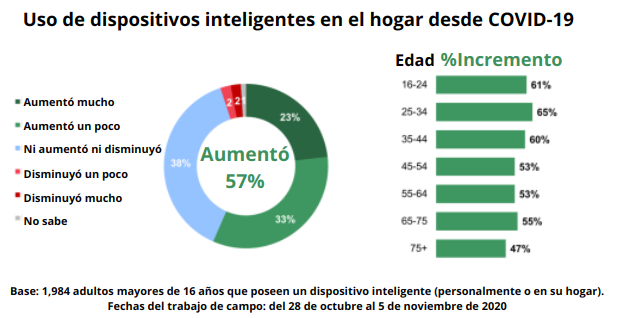
\includegraphics[width=\textwidth]{Imágenes/Uso_de_dispositivos_inteligentes_iot_covid19.png} 
    \caption{Crecimiento del uso de dispositivos inteligentes IoT}
    \label{tab:uso_dispositivos_iot}
\end{table}

\begin{table}[ht]
    \centering
        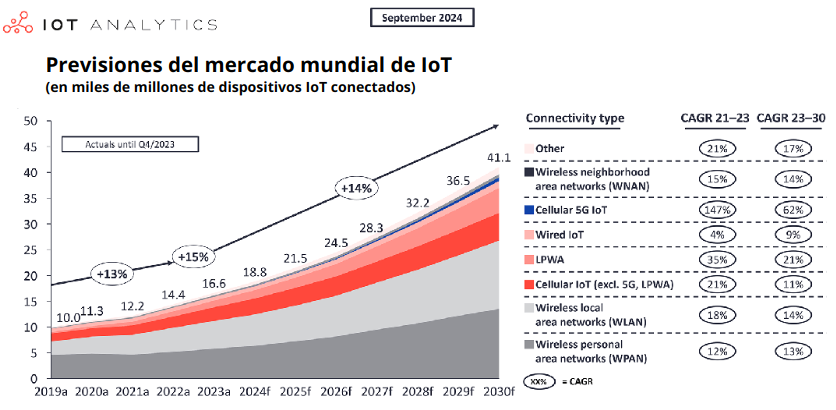
\includegraphics[width=\textwidth]{Imágenes/analytics_IoT_2024.png}
    \caption{IoT 2019-2030}
    \label{tab:iot_analytics}
\end{table}

\begin{table}[ht]
    \centering
        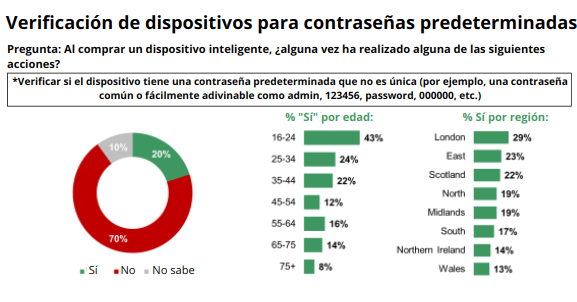
\includegraphics[width=\textwidth]{Imágenes/verificacion_.png}
    \caption{Verificación de dispositivos para contraseñas predeterminadas}
    \label{tab:verificacion_de_dispositivos_para_contraseñas_predeterminadas}
\end{table}


La información proporcionada en los cuadros \ref{tab:uso_dispositivos_iot}, \ref{tab:iot_analytics} y \ref{tab:verificacion_de_dispositivos_para_contraseñas_predeterminadas} brinda herramientas para comprender el crecimiento en el uso y adopción de las tecnologías, así como también los comportamientos de los consumidores en relación con la seguridad del IoT. La inclusión de estos informes pretende proporcionar un marco contextual que resalte la importancia de la seguridad en el desarrollo y adopción de IoT, ofreciendo una perspectiva basada en datos empíricos recolectados directamente de los usuarios finales. \cite{ipsos2021iot} \cite{Sinha2023}

La expansión del ecosistema IoT ha generado el interés de los ciberdelincuentes por sus brechas de seguridad, convirtiéndolo en un mercado fácil y atractivo para explotar. Un informe reciente de la empresa de seguridad Check Point destaca un incremento preocupante en la cantidad de ciberataques dirigidos a dispositivos IoT por sectores.\cite{checkpoint2023iot}. Por su parte la empresa Verizon también reporta incrementos con respecto del año 2023 a 2024, sumando en este último año los ataques a la cadena de suministro en sus estadísticas. Esto quiere decir que los ataques han crecido no sólo en número, sino también en sofisticación \cite{Verizon2023} \cite{Verizon2024} 

\begin{table}[ht]
    \centering
        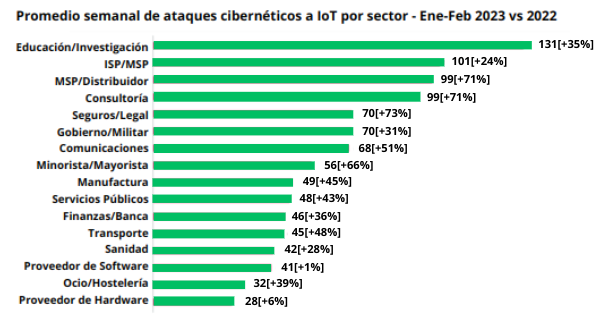
\includegraphics[width=\textwidth]{Imágenes/Promedio_semanal_de_ataques_IoT_2023vs2022.png} 
    \caption{Promedio semanal de ataques IoT 2023 vs 2022 - Check Point}
    \label{tab:promedio_semanal_de_ataques_IoT_2023vs2022}
\end{table}

El incremento en la adopción de dispositivos IoT fue más notorio desde la pandemia COVID-19 y podría creerse que las vulnerabilidades en las tecnologías comenzaron allí, pero esto no es cierto. Las brechas de seguridad vienen de tiempo atrás. Por este motivo quiero citar el trabajo de campo que realizó el Lic. Ricardo Brea, en el cual desarrolló un software integrador homogéneo y seguro para IoT culminado en 2017. Dentro de su investigación se encuentran las brechas acerca de privacidad, contemplando que en Argentina el uso de los datos está regulado por la ley de protección de datos personales (Ley 25.326), pero la jurisprudencia no se adelanta a la tecnología, si no que actúa como consecuencia de ella, y por lo tanto queda desactualizada frente nuevas tecnologías. Destaca también que los dispositivos IoT son susceptibles a ataques cibernéticos al no enviar la información encriptada, lo cual es un riesgo grave teniendo en cuenta que recolectan información de la vida de las personas y algunos poseen actuadores que encienden diversos elementos. Esto significa que un ataque cibernético a un dispositivo IoT puede causar no sólo la perdida de información, sino también una perdida material, o en el peor de los casos causar la muerte si el dispositivo atacado es un elemento que monitorea los signos vitales de una persona enferma. Un caso especial en la seguridad de IoT es cuando un dispositivo es infiltrado y utilizado, sin el conocimiento del usuario, para atacar a un tercero. IoT se convierte en un blanco ideal de ataques informáticos por la gran cantidad de dispositivos que pueden ser “reclutados” a fin de infiltrar y “reclutar” dispositivos para un ataque de denegación de servicio. Este trabajo fue presentado en el XXIV Congreso Argentino de Ciencias de la Computación (CACIC 2018)\cite{brea2018hub}

Las soluciones que existían en 2017/2018 para el uso de IoT no se encontraban integradas, eran inseguras o no eran transparentes en el manejo de la información. En la actualidad transitando el 2024, estas problemáticas siguen vigentes. 

Dentro de la presente investigación, se examinó el artículo ''Regulación mediante "bricking": ordenamiento privado en IoT''\cite{Tusikov2019} , el cual se refiere al deterioro o destrucción deliberada del software con la intención de afectar negativamente la funcionalidad del producto. El artículo argumenta y sostiene que se está empleando bricking a través de la regulación post-compra de bienes conectados a Internet, y que las empresas del “Internet de las Cosas” (IoT) tienen una capacidad injusta para imponer sus políticas preferidas de manera unilateral, automática y remota. Induciendo que el control sobre el software permite por tanto, el control sobre el hardware.

Las brechas de seguridad van dejado el paso abierto a que se consoliden diferentes vulnerabilidades. La empresa líder proveedora de soluciones de seguridad Sectigo, informa la batalla entre los ciberataques y las tecnologías de seguridad.(Cuadro: \ref{tab:evolucion_de_los_ciberataques}), evidenciando el incremento y recurrencia de las Botnets. Según Sectigo la evolución de los ataques a dispositivos IoT se puede dividir en tres eras.(Figura: \ref{fig:sectigo_eras_de_evolucion}).\cite{SectigoNoDate}

\begin{table}[ht]
    \centering
        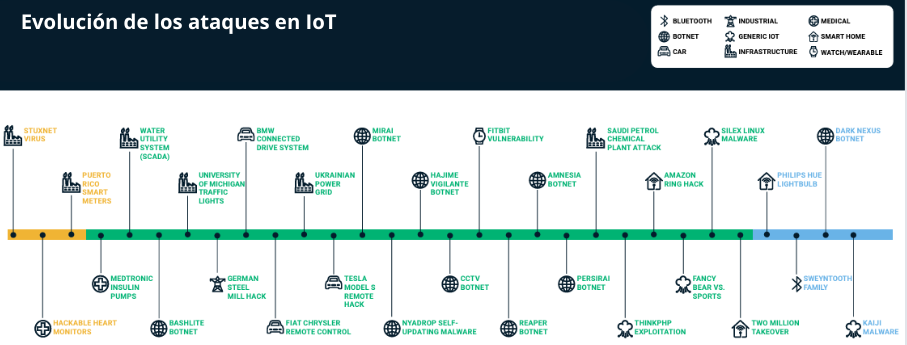
\includegraphics[width=\textwidth]{Imágenes/evolution_of_attacks_iot_sectigo..png} 
    \caption{Evolución de los ciberataques}
    \label{tab:evolucion_de_los_ciberataques}
\end{table}

\begin{figure}[ht]
    \centering
    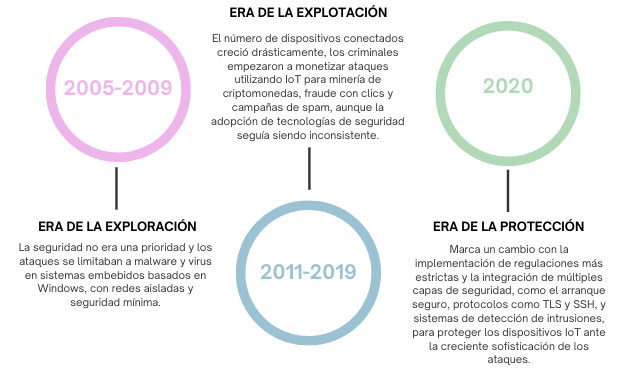
\includegraphics[width=\textwidth]{Imágenes/sectigo_eras_de_evolucion.png}
    \caption{Eras de la evolución de los ciberataques por Sectigo}
    \label{fig:sectigo_eras_de_evolucion}
\end{figure}

Al realizar esta tesis surgió la necesidad de conocer las normativas, regulaciones y entidades existentes para los heterogéneos dispositivos IoT. Dentro de las entidades gubernamentales que defienden el derecho de los consumidores, y reflejan esta defensa en regulaciones se encuentra el ''GDPR'' (General Data Protection Regulation) perteneciente al consejo de la UE(Union Europea), considerada la ley de privacidad y seguridad más estricta del mundo.\cite{consilium_data_protection}

\begin{wrapfigure}{r}{0.35\textwidth} %this figure will be at the right
    \centering
    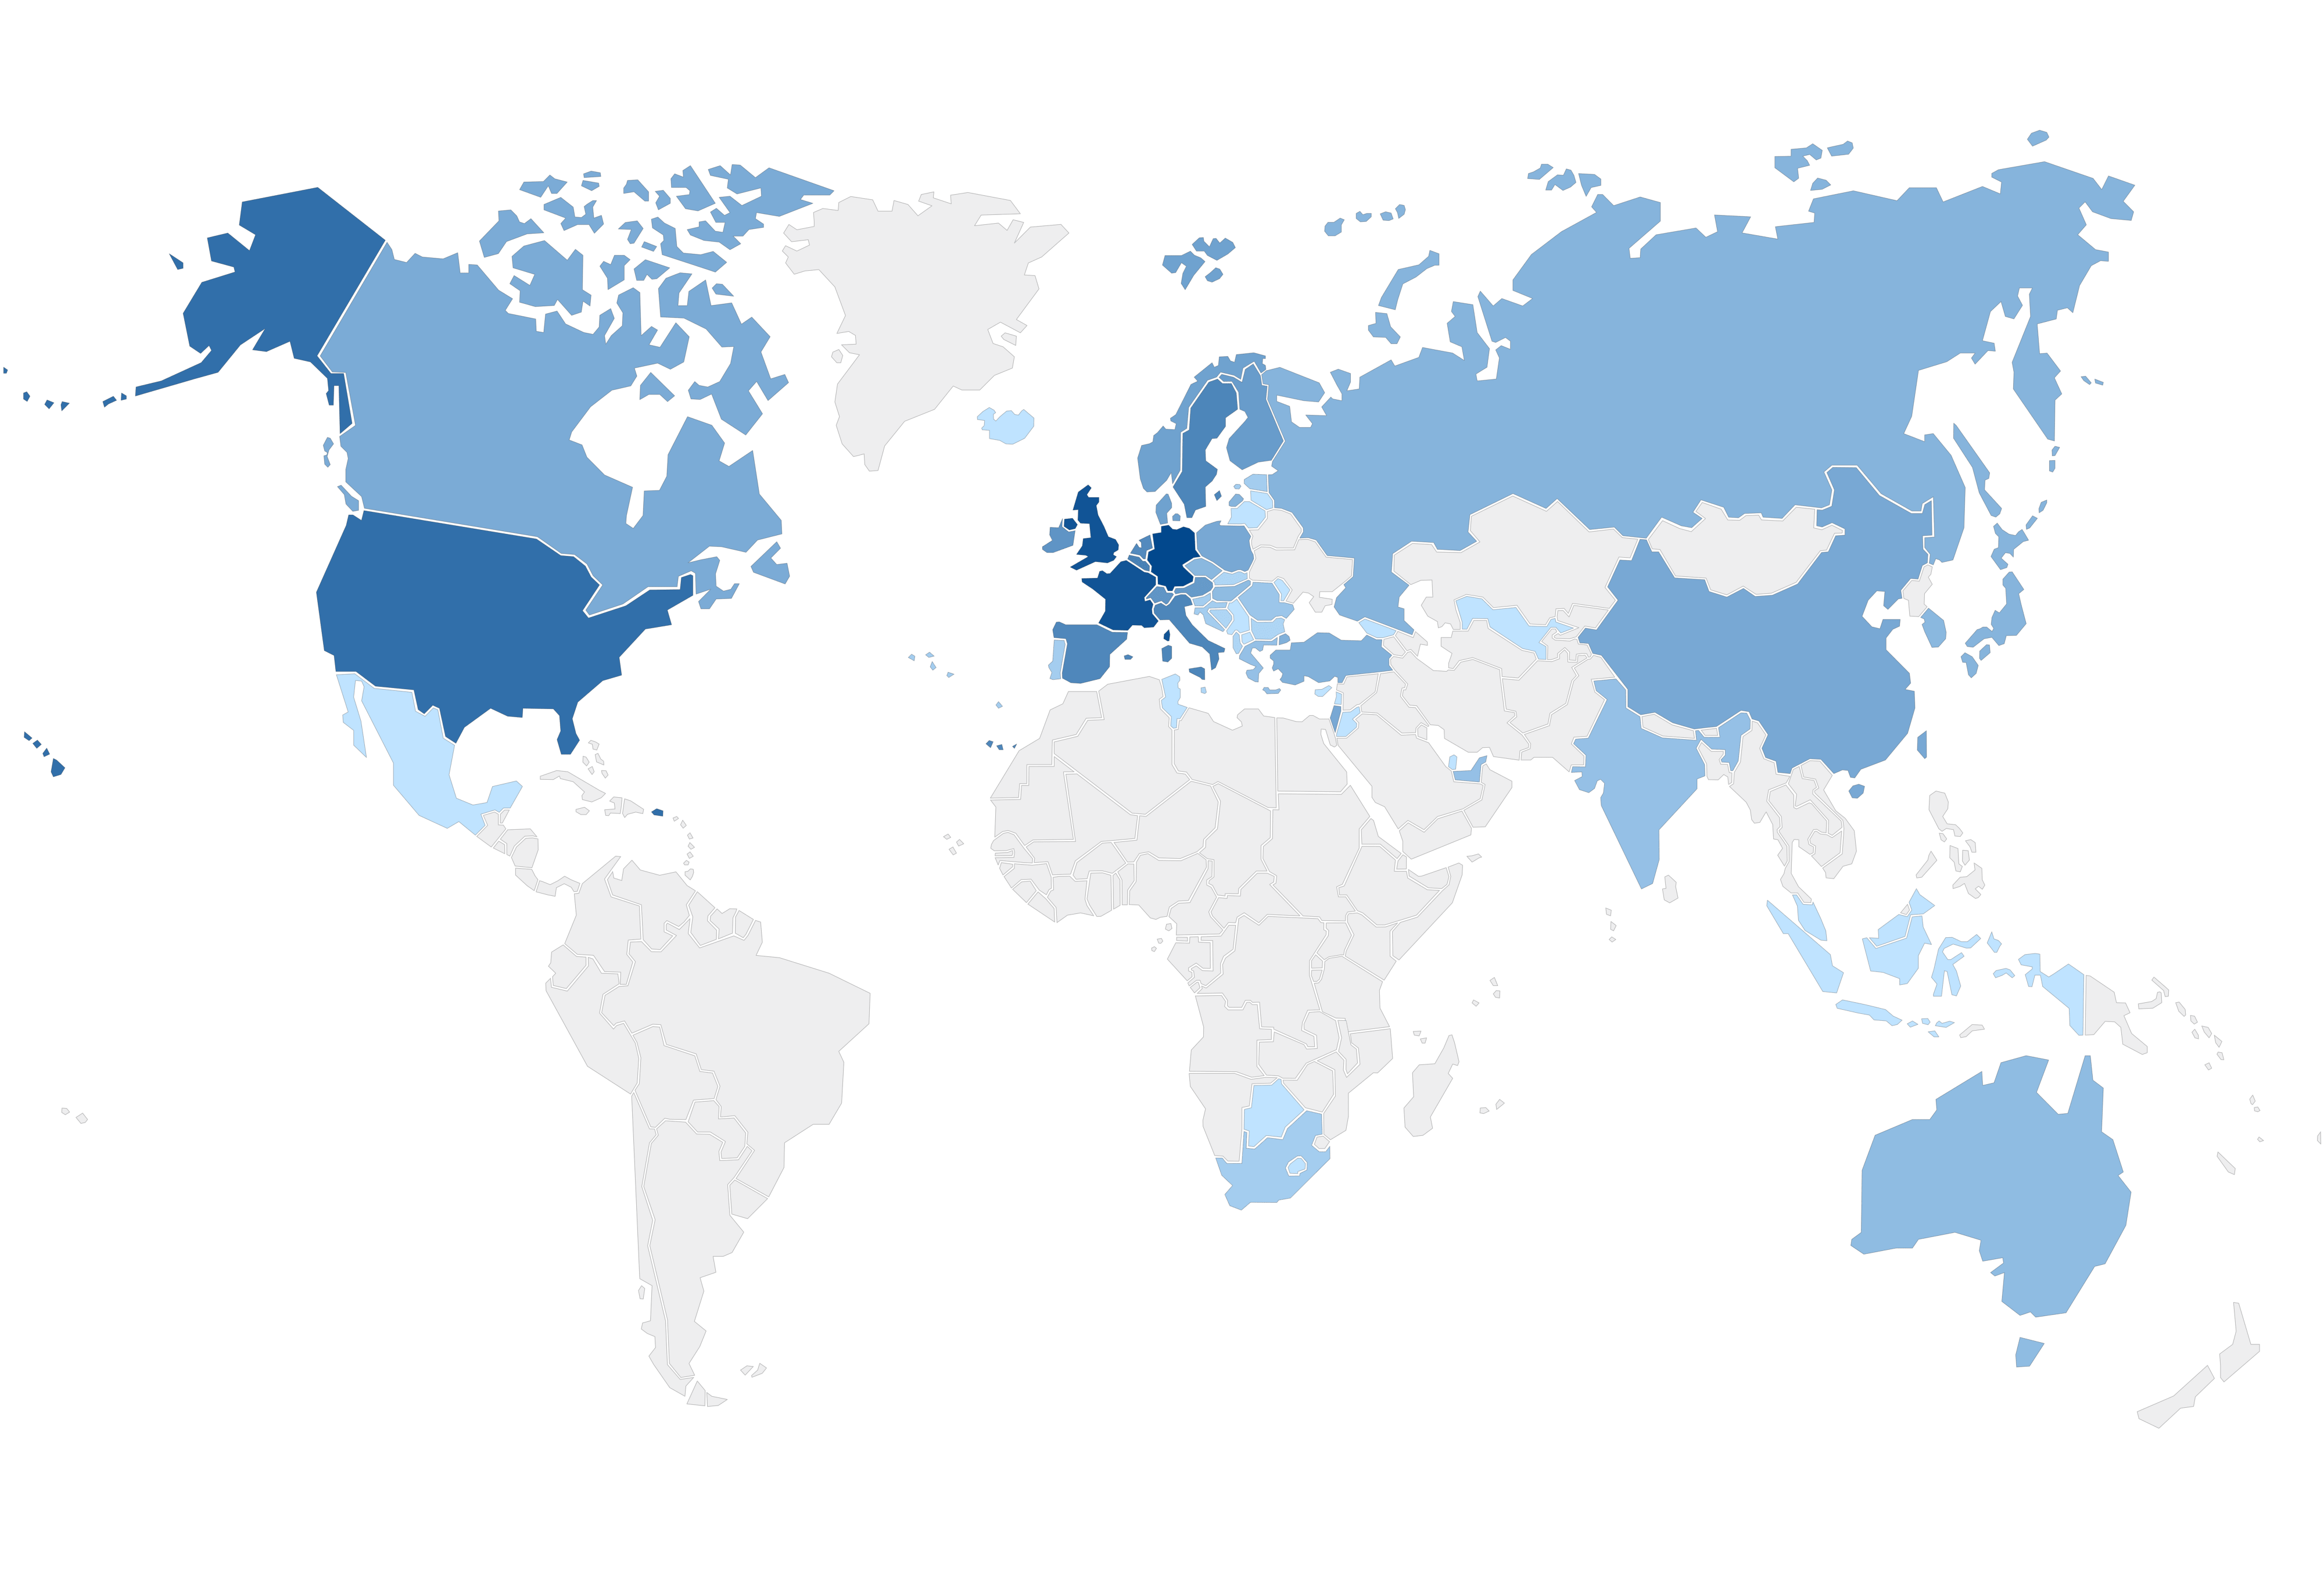
\includegraphics[width=0.35\textwidth]{Imágenes/world-mapETSI.png}
      \caption{Mapa ETSI}
    \label{fig:world-map}
\end{wrapfigure}

El reglamento GDPR actualizó y modernizó la directiva de protección de datos de 1995, fue adoptado en 2016 y entró en vigor el 25 de mayo de 2018, definiendo los derechos fundamentales de los individuos en la era digital, las obligaciones de quienes tratan los datos, los métodos para garantizar el cumplimiento y las sanciones para quienes incumplan las normas. Sin embargo, no cubre todas las particularidades de IoT, es por ello que el ''ETSI'' (European Telecommunications Standards Institute) es el organismo reconocido de normalización regional que se ocupa de las telecomunicaciones, la radiodifusión y otras redes y servicios de comunicaciones electrónicas, con más de 850 organizaciones miembros, que provienen de más de 60 países y cinco continentes.(Figura:\ref{fig:world-map})


ETSI brinda desde el año 2020 un estándar para dispositivos conectados, su objetivo es establecer disposiciones de alto nivel para la seguridad y protección de datos en dispositivos IoT, proporcionando directrices concisas para organizaciones involucradas en el desarrollo y/o fabricación de dispositivos IoT de consumo, indicando cómo implementar las disposiciones de seguridad establecidas.\cite{ETSI_EN303645_2020}.(Cuadro: \ref{tab:resumen_ETSI_directrices})

\begin{table}[ht]
    \centering
        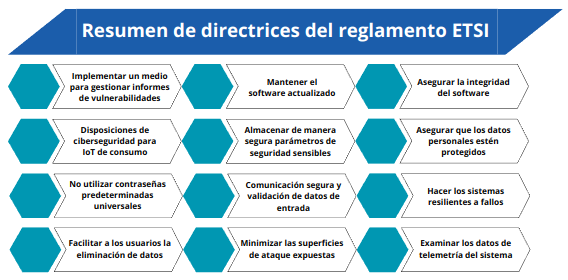
\includegraphics[width=\textwidth]{Imágenes/resumen_directrices_ETSI.png} 
    \caption{Directrices de requerimientos básicos definidos por ETSI 2020}
    \label{tab:resumen_ETSI_directrices}
\end{table}

\begin{wrapfigure}{r}{0.50\textwidth} %this figure will be at the right
   \centering
    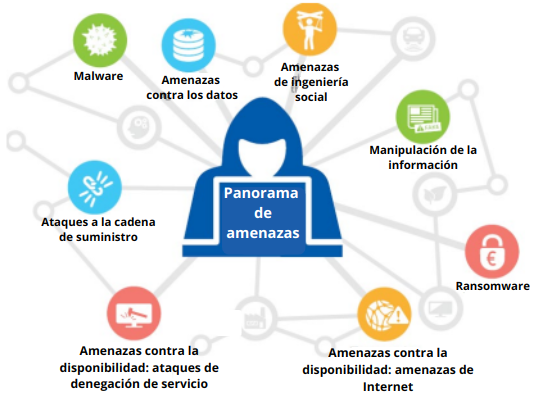
\includegraphics[width=0.50\textwidth]{Imágenes/enisa_panorama_de_amenazas_informe_2023.png}
    \caption{Informe anual ENISA 2023}
    \label{fig:informe-Panorama-de-amenazas-ENISA}
\end{wrapfigure}

La agencia ENISA(European Union Agency for Cybersecurity) es otra organización que colabora en mejorar la ciberseguridad en los estados miembros de la UE y fortalecer la capacidad de respuesta ante incidentes. En su informe anual más reciente sobre el panorama de amenazas de ciberseguridad ENISA identifica las principales amenazas, tendencias, actores maliciosos, técnicas de ataque, analizando su impacto y motivaciones e incluyendo recomendaciones sobre medidas de mitigación.\cite{enisa2023}


Dentro de las organizaciones más relevantes en cuanto a las amenazas y vulnerabilidades se encuentra OWASP(Open Worldwide Application Security Project) una fundación sin fines de lucro que trabaja en mejorar la seguridad en el software. 

OWASP Publica un ranking de las 10 vulnerabilidades más comunes de software que es referenciada en muchos análisis de seguridad.\cite{owaspTopTen}, Así como también enumera y explica, las vulnerabilidades más comunes halladas en los dispositivos IoT.\cite{owasp}

\begin{figure}[ht]
    \centering
    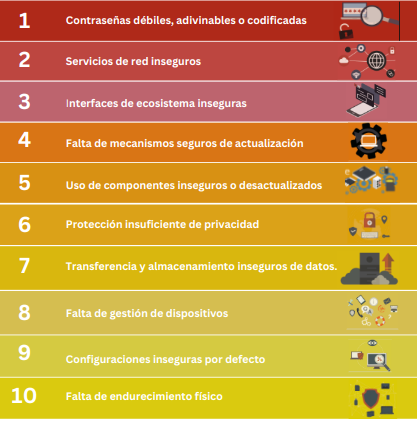
\includegraphics[width=0.7\textwidth]{Imágenes/OWASP_top_10.png}
    \caption{Resumen OWASP 2018 IoT Top10}
    \label{fig:OWASP_2018_IoT_Top10}
\end{figure}

Dado que las regulaciones GDPR y ETSI datan de algunos años atrás se investigó acerca de la actualidad para conocer si han surgido nuevas soluciones a las problemáticas de IoT. Existe un trabajo de investigación y práctica que implementa SecOps realizado en 2023 abordando los desafíos mediante técnicas combinadas de seguridad, operaciones y buenas prácticas. Este trabajo da muestras de las mejoras y mitigaciones que se pueden lograr en dispositivos ya existentes si se aplican las medidas necesarias. Si bien, los desafíos eran los mismos de años atrás(figura: \ref{fig:iot_challenges}), utilizar un enfoque moderno ha mejorado de manera contundente los resultados.\cite{jorgensen2023secops}

\begin{figure}[ht]
    \centering
    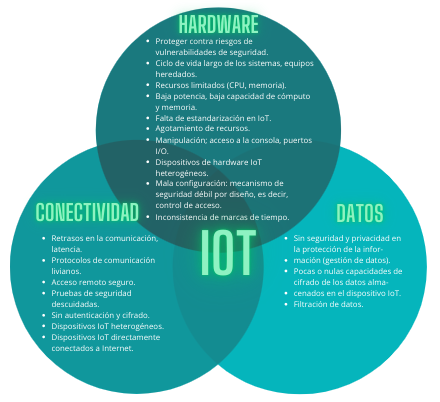
\includegraphics[width=0.9\textwidth]{Imágenes/desafios_iot_por_capas.png}
    \caption{Desafíos de seguridad existentes en 2023 para IoT}
    \label{fig:iot_challenges}
\end{figure}

La escasez de soluciones y mitigaciones tempranas a las vulnerabilidades de las tecnologías IoT, que avanzan a mayor velocidad que las medidas adecuadas de contención en temas referentes a la seguridad en los dispositivos de comercialización, se convierten en la motivación necesaria para realizar el presente trabajo, proponiendo la implementación de DevSecOps como medida cautelar y mitigatoria de los desafíos emergentes.